\documentclass[a5paper,12pt,twoside]{book}

\usepackage[tmargin=20mm,bmargin=25mm,lmargin=20mm,rmargin=20mm]{geometry} % Formato de página

\usepackage[output-decimal-marker={,}]{siunitx} % Unidades del SI
    \sisetup{per-mode = fraction}
    \DeclareSIUnit{\rpm}{rpm}
    \DeclareSIUnit{\atmosphere}{atm}

\usepackage[framemethod=TikZ]{mdframed} % Define \begin{mdframed}[style=MyFrame1]

    \mdfdefinestyle{MyFrame1}
    {linecolor=black!80!gray,
    outerlinewidth=0.5pt,
    roundcorner=0pt,
    innertopmargin=15pt,
    innerbottommargin=20pt,
    innerrightmargin=15pt,
    innerleftmargin=15pt,
    backgroundcolor=gray!30!white}

    \mdfdefinestyle{MyFrame2}
    {linecolor=white,
    outerlinewidth=0.5pt,
    roundcorner=10pt,
    innertopmargin=15pt,
    innerbottommargin=20pt,
    innerrightmargin=15pt,
    innerleftmargin=15pt,
    backgroundcolor=gray!20!white}

\usepackage{graphicx}
    \graphicspath{{./images/}} % Define \graphicspath{{dir1}{dir2}} para incluir imágenes que estén en los directorios dir1 y dir2

\usepackage[spanish]{babel}  % Traducciones y abreviaturas
\usepackage{amssymb}  % Símbolos y tipografía matemáticos
\usepackage{amsmath}  % Formato y estructura matemáticos
\usepackage{esint} % Define \oiint para integrales cerradas y acomoda \iiint
\usepackage{hyperref}  % Referencias cruzadas
\usepackage{fancyhdr}  % Encabezado y pie
\usepackage{graphicx}  % Define \includegraphics
\usepackage{pdfpages} % Define \includepdf
\usepackage{multicol} % Entorno de formato en columnas
\usepackage{comment} % Comenta todo entre \begin{comment} \end{comment}
% COMANDOS DE FORMATO
\newcommand{\sub}[2]{{{#1}_\textsl{{#2}}}} % #1 subíndice #2 (Usado cuando #2 es $texto$)
\newcommand{\scale}[2]{\text{\scalebox{#1}{$#2$}}} % Aplicar factor de escala #1 a la ecuación #2
\newcommand{\cusTi}[1]{\noindent\textbf{#1}} % Título de definiciones, propiedades y ejemplos
\newcommand{\cusTe}[1]{\vspace{2mm}\\\text{\hspace{\the\parindent}}#1} % Descripción de definiciones, propiedades y ejemplos
\newcommand{\noTi}[1]{\text{\hspace{\the\parindent}}#1} % Descripción de MyFrame1 que no tenga título
\newcommand{\concept}[1]{\vspace{1ex} \textsc{#1}} % Subtítulos sin jerarquía
\newcommand{\braces}[1]{{ \left\{ {#1} \right\} }} % #1 entre llaves
\newcommand{\sqb}[1]{{ \begin{bmatrix} #1 \end{bmatrix} }} % #1 entre corchetes
\newcommand{\bb}[1]{\left(#1\right)} % #1 entre paréntesis
\newcommand{\sfrac}[2]{#1/#2} % Fracciones #1/#2 para reemplazar el (muy lento) \usepackage{xfrac}
\newcommand{\captionSpace}{-0.8cm} % Espacio entre figuras y pie de foto

% COMANDOS PARA NOTACIÓN DE FUNCIONES
\newcommand{\barrow}[3]{\begin{bmatrix} \left. #1 \right|_{#2}^{#3} \end{bmatrix}} % Regla de Barrow de #1 para los extremos de integración #2 y #3
\newcommand{\fx}[2][f]{#1 \hspace{-0.5mm} \left( #2 \right)} % #1 en función de #2 con paréntesis
\newcommand{\ffx}[2][f]{#1 \hspace{-0.5mm} \begin{bmatrix} #2 \end{bmatrix}} % #1 en función de #2 con corchetes
\newcommand{\intProd}[2]{<\hspace{-0.8mm}#1,#2\hspace{-0.8mm}>} % Producto interno entre #1 y #2
\newcommand{\comb}[2]{\begin{pmatrix} {#1}\\{#2} \end{pmatrix}} % Combinatorio n=#1, m=#2
\newcommand{\media}[2]{\underset{#2}{\sub{#1}{med}}} % #1 media entre #2
\newcommand{\norm}[1]{{\left| {#1} \right|}} % Módulo de #1
\newcommand{\nnorm}[1]{{\left|\left| {#1} \right|\right|}} % Norma de #1
\newcommand{\trans}[1]{#1^*} % Matriz transpuesta de #1
\newcommand{\conj}[1]{\overline{#1}} % Conjugado de #1
\newcommand{\ave}[1]{\bar{#1}} % Valor promedio de #1
\newcommand{\rms}[1]{{\sub{#1}{ef}}} % Valor eficaz de #1
\newcommand{\peak}[1]{{\sub{#1}{pk}}} % Valor pico de #1

% COMANDOS PARA NOTACIÓN DE ELEMENTOS Y OPERADORES
\newcommand{\class}[1][1]{\mathcal{C}^{#1}} % Clase o cantidad de derivadas parciales contínuas
\newcommand{\versor}[1]{\hat{#1}} % Vector unitario #1
\newcommand{\fasor}[1]{\check{#1}} % Fasor #1
\newcommand{\iVer}{\versor{\imath}} % i versor
\newcommand{\jVer}{\versor{\jmath}} % j versor
\newcommand{\kVer}{\versor{k}} % k versor
\newcommand{\eVer}{\versor{\textbf{e}}} % Versor canónico
\newcommand{\tang}{\textbf{t}} % Vector tangente
\newcommand{\setO}{\varnothing} % Conjunto vacío
\newcommand{\setN}{\mathbb{N}} % Conjunto de los números naturales
\newcommand{\setZ}{\mathbb{Z}} % Conjunto de los números enteros
\newcommand{\setR}{\mathbb{R}} % Conjunto de los números reales
\newcommand{\setI}{\mathbb{I}} % Conjunto de los números imaginarios
\newcommand{\setC}{\mathbb{C}} % Conjunto de los números complejos
\newcommand{\iu}{\mathrm{i}\mkern1mu} % Unidad imaginaria o número i
\newcommand{\setV}{\mathbb{V}} % Espacio vectorial V
\newcommand{\setW}{\mathbb{W}} % Espacio vectorial W
\newcommand{\setK}{\mathbb{K}} % Cuerpo K
\newcommand{\ith}{i} % Valor i-ésimo para sumatorias y permutadores
\newcommand{\jth}{j} % Valor j-ésimo para sumatorias y permutadores
\newcommand{\kth}{k} % Valor k-ésimo para sumatorias y permutadores
\newcommand{\nth}{n} % Valor n-ésimo para sumatorias y permutadores
\newcommand{\Nth}{N} % Valor N-ésimo para sumatorias y permutadores
\newcommand{\mth}{m} % Valor m-ésimo para sumatorias y permutadores
\newcommand{\dif}{\textsl{d}} % Diferencial
\newcommand{\grad}{\Vec{\nabla}} % Gradiente a fin
\newcommand{\absurd}{\bot} % Absurdo o contradicción
\newcommand{\tq}{\hspace{1ex} \big/ \hspace{1ex}} % tal que
\DeclareMathOperator{\sgn}{sgn} % Función signo
\DeclareMathOperator{\artan}{artan} % Arco tangente
\DeclareMathOperator{\sinc}{sinc} % Seno de x sobre x
\DeclareMathOperator{\proy}{proy} % Proyección ortogonal
\DeclareMathOperator{\Nu}{Nu} % Núcleo
\DeclareMathOperator{\im}{Im} % Imagen
\DeclareMathOperator{\ran}{ran} % Rango
\DeclareMathOperator{\bi}{Bi} % Variable aleatoria binomial
\DeclareMathOperator{\be}{Be} % Variable aleatoria de Bernoulli
\DeclareMathOperator{\geo}{G} % Variable aleatoria geométrica
\DeclareMathOperator{\hip}{H} % Variable aleatoria hipergeométrica
\DeclareMathOperator{\po}{Po} % Variable aleatoria de Poisson
\DeclareMathOperator{\uni}{U} % Distribución uniforme
\DeclareMathOperator{\ex}{exp} % Distribución exponencial
\DeclareMathOperator{\nor}{N} % Distribución normal
\DeclareMathOperator{\ecm}{ECM} % Error cuadrático medio (MSE)

% COMANDOS PARA NOTACIÓN DE CONSTANTES Y MAGNITUDES
\newcommand{\weight}{\textsl{p}} % Peso
\newcommand{\xyz}{\vec{r}\hspace{0.05cm}} % Trayectoria [x(t),y(t),z(t)]
\newcommand{\cstcoulomb}{k_e} % Constante de Coulomb

% ENTORNOS DE NUMERACIÓN
\newtheorem{defn}{{Definición}}[chapter]
\newtheorem{prop}{{Propiedad}}[chapter]
\newtheorem{example}{{Ejemplo}}[chapter]

% ENTORNOS DE FORMATO
\newenvironment{formatI}{\vspace{1ex}\par\small\sffamily} % Consignas de ejemplos


\begin{document}

\pagestyle{fancy}
\fancyhf{}
\chead{\scriptsize \nouppercase\rightmark}
\cfoot{\scriptsize \thepage}
\pagenumbering{gobble}
\renewcommand{\headrulewidth}{0pt}

\frontmatter
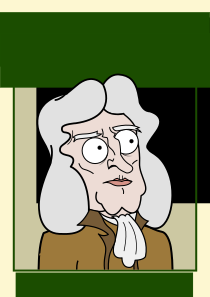
\includepdf{./images/cover/cover-front}

\begin{center}

    \begin{Huge}
    \textbf{Súper libro de Física}
    \end{Huge}

    \vspace{1cm}
    \textbf{Primera edición v0.1}
    \vspace{2cm}

    \begin{Large}
        Malvicino, Maximiliano R. \\
        Bosio, Federico A.
    \end{Large}

\end{center}

\clearpage
\noindent
\textbf{Prefacio}

La versión digital más reciente de este texto puede ser descargada gratuitamente de
\begin{center}
    \url{https://github.com/mrmalvicino/super-libro-de-fisica}
\end{center}

\renewcommand{\spanishappendixname}{Anexo}
\tableofcontents

\mainmatter
\pagenumbering{arabic}


\chapter{Cinemática}

\emph{La cinemática es el estudio del movimiento.}
El movimiento suele describirse mediante tres magnitudes: posición, velocidad y aceleración.
A grandes rasgos, estas magnitudes se comprenden como sigue.
\begin{itemize}
    \item La posición indica dónde está lo que se mueve.
    \item La velocidad indica qué tan rápido se mueve.
    \item La aceleración indica con qué fuerza se mueve.
\end{itemize}

\begin{mdframed}[style=MyFrame2]
    \begin{example}
        \label{eg:mag}
    \end{example}
    \cusTi{Magnitudes cinemáticas}

    Para un auto en el kilómetro 10 de la Ruta Provincial 4, cuyo velocímetro marca \SI{60}{\kilo\meter/\hour}, y cuyo conductor pisa bruscamente el freno:
    \begin{itemize}
        \item La posición del auto se indica en el ``mojón kilométrico'' que, en este caso, está a \SI{10}{km} del lugar en el que nace la ruta.
        \item La velocidad está en los controles indicadores del auto, es decir, el velocímetro, que marca \SI{60}{\kilo\meter/\hour}.
        \item La aceleración está relacionada con la fuerza que sienten los pasajeros del auto cuando el conductor pisa el freno.
        La aceleración de frenado de un automóvil común ronda los \SI{5}{\meter/\second\squared}.
    \end{itemize}

    \begin{center}
        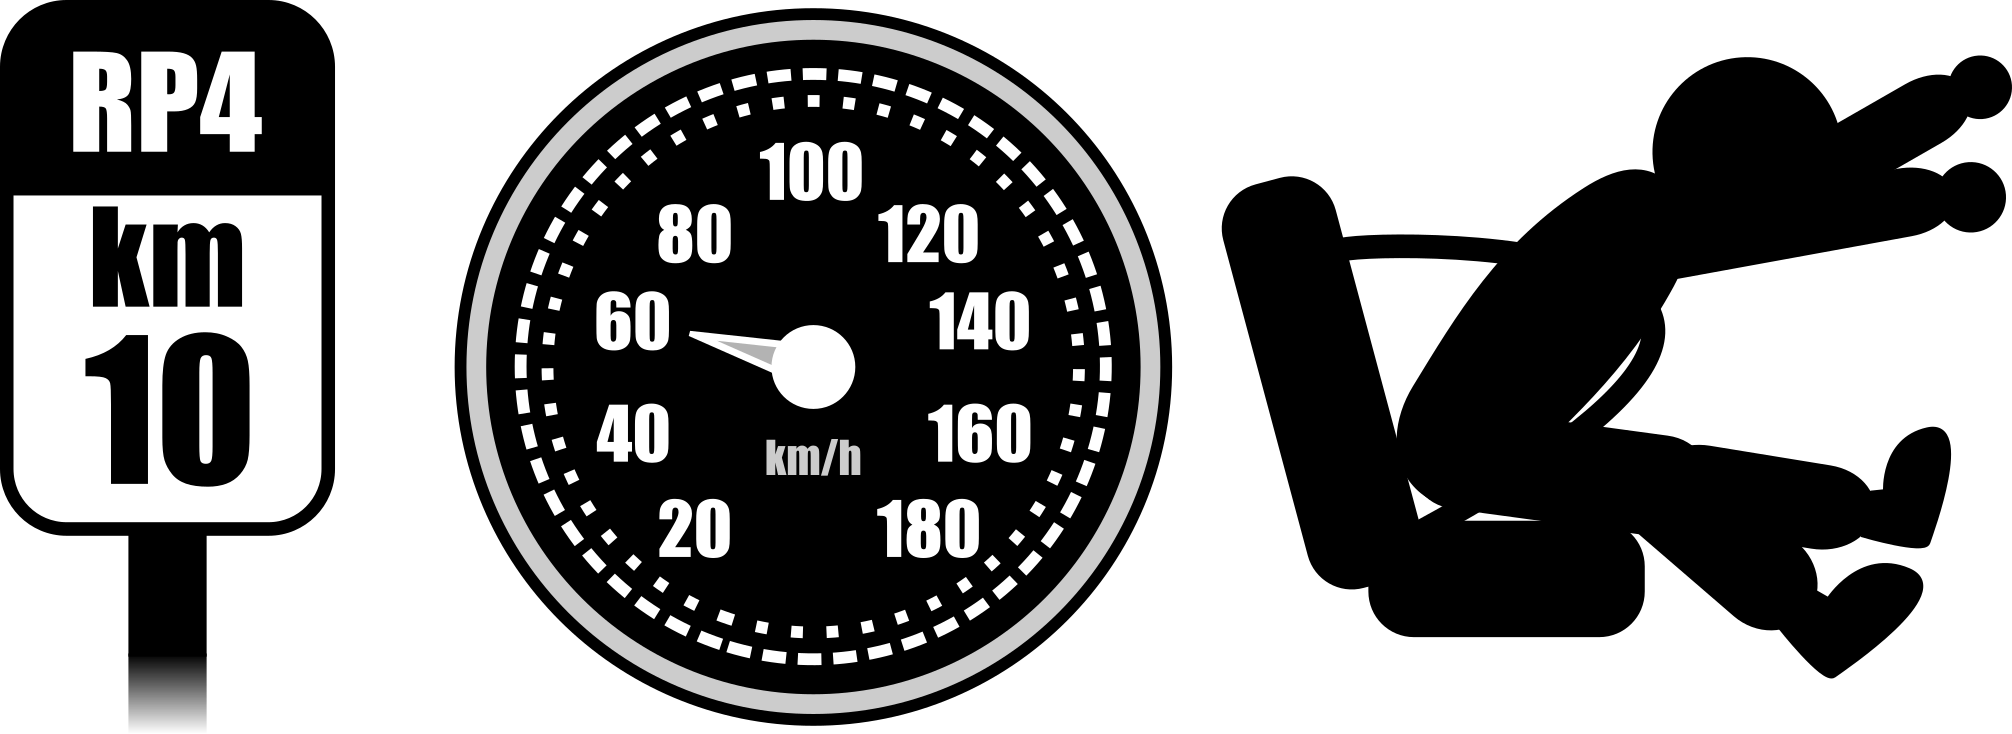
\includegraphics[width=\linewidth]{cinematica-mojon.png}
    \end{center}
\end{mdframed}

En este capítulo, van a estudiarse distintos movimientos que involucran las tres magnitudes.
Cabe destacar que sólo se estudian los movimientos en sí, y no sus causas, que se verán en capítulos posteriores.

\section{Posición, trayectoria y desplazamiento}

La posición se modela matemáticamente como un vector en el espacio, cuyas coordenadas se expresan en un sistema de referencia determinado. En su forma más general, el vector posición se define como sigue.

\begin{mdframed}[style=MyFrame1]
    \begin{defn}
        \label{defn:position}
    \end{defn}
    \cusTi{Función de posición}
    \begin{equation*}
        \xyz(t) = \begin{bmatrix} x(t) & y(t) & z(t) \end{bmatrix}
    \end{equation*}
\end{mdframed}

Todas las coordenadas son funciones del tiempo, lo cual se pone de manifiesto en las $t$ entre paréntesis que aparecen en la notación.
Las relaciones que las componentes del vector posición tienen con la variable $t$ se llaman \emph{ecuaciones horarias}, \emph{ecuaciones de movimiento}, o \emph{ecuaciones paramétricas}.

A veces es necesario usar un vector pero basta con que tenga dos de las tres dimensiones espaciales. La posición de movimientos en dos dimensiones suele denotarse entonces como $\xyz(t)=\sqb{x(t)&y(t)}$ o lo que es lo mismo $\xyz(t)=x(t)\,\iVer + y(t)\,\jVer$ siendo $\iVer$ y $\jVer$ los versores canónicos.

En muchos casos (como en el ejemplo \ref{eg:mag} del auto en la ruta), interesa solamente la distancia a una referencia (el número escrito en el cartel) y en ves de usar un vector $\xyz(t)$ se trabaja con un escalar, generalmente denotado $x(t)$.

Podemos referirnos a una única posición de un cuerpo en un instante de tiempo en particular. Esto es, evaluar dicho instante $t_\ith$ en $\xyz(t)$ para obtener un vector que tiene valores numéricos fijos en sus componentes.

O bien podemos referirnos a todo el recorrido, dado por la imagen de $\xyz(t)$ que traza las sucesivas posiciones por las que pasa el cuerpo conforme transcurre el tiempo. A este recorrido se lo llama \emph{trayectoria}. La trayectoria es el espacio geométrico que ocupan todas las posiciones de un cuerpo en movimiento, dadas por $\xyz(t)$.

En el siguiente gráfico se observa que una \emph{trayectoria} es el conjunto de posiciones sucesivas por las que pasa un cuerpo, mientras que $P_{t_\ith}=\sqb{x(t_\ith)&y(t_\ith)}$ es una de las posiciones que toma el cuerpo a lo largo de su trayectoria.

\begin{center}
    \vspace{-6cm}
    \def\svgwidth{\linewidth}
    \input{./images/cinematica-trayect-1.pdf_tex}
    \vspace{-6cm}
\end{center}  

Para toda trayectoria o fragmento de trayectoria se puede definir el desplazamiento, que es el vector que une el punto inicial con el final. Esto es, la resta entre ambos vectores:

\end{document}
